% Status überarbeitet
% Status Zweitkorrekt 

%TODO: Zitiere mar_02_archeology.pdf  => Instead of hiding in a “duck blind” (warum high level)

\section{Analyse der statischen Ist-Architektur}

\subsection{Reverse Engineering}
Da die Ist-Architektur des FreeDesign-Editors zuvor kaum dokumentiert war, musste die aktuelle Architektur zunächst rekonstruiert werden. 
Dies wird als \emph{Reverse Engineering} bezeichnet und hat, laut der Definition von Chikofsky und Cross (\citeyear[S. 13-17]{Chikofsky1990}), zwei Ziele: 
\begin{itemize}
    \item Die Darstellung des Softwaresystem in einer abstrakten Form. 
    \item Die Identifikation der Komponenten eines Softwaresystems und ihre Beziehungen untereinander. 
\end{itemize}
Das Reverse-Engineering der Ist-Architektur des FreeDesign-Editor bezieht sich auf den Projektzustand vom 11. Januar 2020. 

\subsection{Darstellung des Softwaresystems}
Das Ziel war eine Form der Darstellung des Softwaresystems zu finden, die das Identifikation der Komponenten und ihrer statischen Zusammenhänge unterstützt.

\subsubsection{Das {dependency-cruiser}-Werkzeug}
Das Reverse Engineering kann durch den Einsatz von Analyse-Werkzeugen unterstützt werden, wobei üblicherweise ein einzelnes Werkzeug nicht alle Analyse-Aufgaben übernehmen kann \autocite[vgl.][381]{Bass2013}.  

Für die Visualisierung der Ist-Architektur wurde das Werkzeug \emph{dependency-cruiser}\footnote{Das Werkzeug \emph{dependency-cruiser} ist unter \url{https://github.com/sverweij/dependency-cruiser} veröffentlicht.}, welches von Sander Verweij entwickelt wurde, in der Version v9.22.0 eingesetzt. 
Das Werkzeug untersucht das Verzeichnis, in dem der Quelltext eines TypeScript-Projektes enthalten ist und visualisiert die Struktur des Quelltextes als Abhängigkeitsgraph. Weiterhin können Regeln für die Abhängigkeiten der Komponenten angelegt werden, die durch das Werkzeug validiert, Verstöße gekennzeichnet und als Report ausgeben werden können \autocite[vgl.][]{Verweij:Dependency}. 

Das \emph{dependency-cruiser}-Werkzeug ist ein Programm für die Kommandozeile, welches mit unterschiedlichen Argumenten aufgerufen werden kann \autocite[vgl.][]{Verweij:CLI}.

\subsubsection{Konfiguration des dependency-cruiser-Werkzeug}
Für alle Analysen mit dem dependency-cruiser-Werkzeug wurde dieselbe Konfigurationsdatei angelegt, welche im Anhang unter \emph{W1\_dependency-cruiser-konfiguration.json} enthalten ist. Diese wurde beim Aufruf des Programms durch die Angabe des Argumentes \lstinline|--config| eingebunden.
\begin{lstlisting}[language={sh}, label=depcruise-config, caption=Aufruf des \emph{dependency-cruiser} mit eingebundener Konfigurationsdatei]
    npx depcruise --config W1_dependency-cruiser-konfiguration.json src
\end{lstlisting}
Die Konfigurationsdatei liegt im JSON-Format vor. 

Das JSON-Format ist ein sprachunabhängiges Format zum Austausch von Informationen, welches auf strukturierten Text basiert. Der Text ist ein serialisiertes Objekt oder Array, deren Werte vom Datentyp Objekt, Array, Nummer oder eine Zeichenkette sein können. Weiterhin sind die Literale \lstinline|null|, \lstinline|true| und \lstinline|false| valide Wertzuweisungen \autocite[vgl.][]{JSON:Einführung}.  

Die Konfigurationsdatei besteht aus einem JSON-Objekt mit der, in Listing \ref{list:dc-config} abgebildeten, Struktur.
\begin{lstlisting}[language=sh, label=list:dc-config, caption=Struktur der Konfiguration für das dependency-cruiser-Werkzeug]
{
    "options": {
        "tsConfig": Object,
        "webpackConfig": Object,
        "reporterOptions": Object,
        "exclude": { "path": Array }
    },
    "allowed": Array,
    "forbidden": Array
}
\end{lstlisting}

% options
Die Eigenschaften \lstinline|tsConfig| und \lstinline|webpackConfig| des \lstinline|options|-Objekts enthalten Informationen über die Konfiguration des TypeScript-Projekts. Über die Eigenschaft reporterOptions konnte Einfluss auf das Aussehen der Abhängigkeitsgraphen genommen werden. Für die Eigenschaft \lstinline|exclude| wurde ein Array mit Pfadangaben, die von der Analyse ausgeschlossen werden sollten, angelegt. Dies betraf Abhängigkeiten zu externen Javascript-Bibleotheken, die für die interne Architektur keine Rolle spielen sowie Daten für Unit-Tests und CSS-Dateien. 

% forbidden & allowed
Die Eigenschaften \lstinline|forbidden| und \lstinline|allowed| enthalten die Regeln zur Validierung der Abhängigkeiten zwischen den Quelltextkomponenten. 
Beide Arrays enthalten eine Liste von Objekten, deren Grundstruktur durch Listing \ref{list:dc-relation} dargestellt wird.

\begin{lstlisting}[language=sh, label=list:dc-relation, caption=Struktur der Objekte für die Arrays \lstinline|forbidden| und \lstinline|allowed|]
{
    "from": { "path": String | Array }
    "to": { "path": String | Array }
}
\end{lstlisting}
Der Eigenschaft \lstinline|path| kann entweder ein einzelner regulärer Ausdruck oder ein Array aus regulären Ausdrücken zugewiesen werden. 
Auf Basis der Ausdrücke untersucht das Werkzeug \lstinline|import|-Anweisungen innerhalb von TypeScript-Dateien. Dabei bezieht sich die Eigenschaft \lstinline|path| in \lstinline|from| auf importierende Dateien und die Eigenschaft \lstinline|path| in \lstinline|to| auf importierte Dateien \autocite[vgl.][]{Verweij:Rules}.

Die genaue Funktionsweise wird in Listing \ref{list:depcruise-example} anhand eines Beispiels illustriert und anschließend erläutert.
\begin{lstlisting}[language={sh}, label=list:depcruise-example, caption=Beispiel einer Abhängigkeitesrelation]
{
    "from": { "path": "^src/services" },
    "to": { "path": [
        "^src/core",
        "^src/store",
        "^src/actions/types/ApiActionTypes.ts",
        "^src/actions/types/ProductApiActionTypes.ts",
        "^src/actions/types/GuiActionTypes.ts"
    ]}
},
\end{lstlisting}
Das Beispiel stammt aus dem \lstinline|allowed|-Array und erlaubt somit, dass Quelltext der innerhalb des Ordners \lstinline|src/services| liegt, auf Quelltext innerhalb der in \lstinline|to| angeben Pfade zugreifen darf. 
Somit ist beispielsweise die Importangabe \newline  
\glqq\lstinline|import ApiRoutes from '../../core/api/ApiRoutes';|\grqq \newline
innerhalb der Datei \lstinline|src/services/designService/CustomerDesignService.ts| valide.

Den Objekten können noch weitere Eigenschaften zugewiesen werden, für das \lstinline|forbidden|-Array wurden lediglich noch die Möglichkeiten der Namenszuweisung und der Zuweisung des Schweregrades eines Fehlers genutzt. Für den Schweregrad wurden die Grade \emph{Warnung} (\lstinline|warn|) und \emph{Fehler} (\lstinline|error|) genutzt.

Zunächst wurden Abhängigkeiten, für die innerhalb des Teams Konsens bestand, dass es sie grundlegend nicht geben darf, in das \lstinline|forbidden|-Array eingetragen. Während der Analyse der Ist-Architektur wurden die bestehenden Abhängigkeiten überprüft und alle Abhängigkeiten, die für valide befunden wurden, in das \lstinline|allowed|-Array aufgenommen. Da es für die Abhängigkeiten nur lose, mündlich kommunizierte Regeln gab, konnten nur wenige Einschränkungen der Abhängigkeiten tatsächlich getroffen werden.  

Das \lstinline|forbidden|-Array wurde außerdem durch die Einträge 
\lstinline|no-orphans| und \lstinline|no-circular| ergänzt.

Der Eintrag \lstinline|no-orphans| dient zum Aufdecken von ungenutzten Quelltextbestandteilen, was für die Entwicklung der Soll-Architektur wichtig war.

Mit Hilfe der Option \lstinline|no-circular| konnten zyklische Abhängigkeiten aufgedeckt werden.

Anlehnend an Lilienthal (\citeyear[vgl.][88 - 90]{Lilienthal2019}) greifen bei zyklischen Abhängigkeiten Komponenten gegenseitig aufeinander zu und bedingen sich somit gegenseitig. 

\begin{figure}[H]
    \centering
    \caption{Beispiele für Abhängigkeiten basierend auf Lilienthal}
    \label{fig:exampleCircular}
    \begin{subfigure}[b]{.3\textwidth}
        \centering
        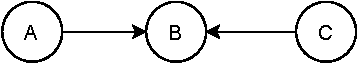
\includegraphics[width=.9\textwidth]{diagrams/Methoden/Circular-Example-C.pdf}
        \caption{ohne Zyklus}
        \label{fig:circularA}
    \end{subfigure}
    %\qquad
    \begin{subfigure}[b]{.3\textwidth}
        \centering
        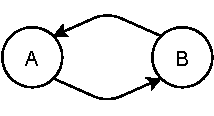
\includegraphics[width=.6\textwidth]{diagrams/Methoden/Circular-Example-A.pdf}
        \caption{mit Zyklus}
        \label{fig:circularB}
    \end{subfigure}
    %\qquad
    \begin{subfigure}[b]{.3\textwidth}
        \centering
        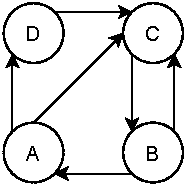
\includegraphics[width=.5\textwidth]{diagrams/Methoden/Circular-Example-B.pdf}
        \caption{Zyklusgruppe}
        \label{fig:circularC}
    \end{subfigure}
\end{figure}
In Abbildung \ref{fig:circularA} sind zwei zyklusfreie Abhängigkeiten illustriert, wobei A und B auf C zugreifen. Somit sind A und B von C entkoppelt. Eine Änderung an C hat Einfluss auf A und B, jedoch hat eine Änderung in A oder B keinen Einfluss auf C. Dadurch sind Abhängigkeiten leicht verständlich und problemlos erweiterbar. 
Auch lässt sich B isoliert von A und C testen. Für Tests von A und C kann B einfach simuliert werden.

Treten hingegen Zyklen in den Abhängigkeiten, wie in Abbildung \ref{fig:circularB} und \ref{fig:circularC} illustriert, auf, verringert sich die Verständlichkeit des Quelltextes und er lässt sich nur schwer ändern. Weiterhin lassen sich Komponenten in Zyklen schwer mit Unit-Tests testen und sind fehleranfällig \autocite[vgl.][116-117]{Martin2018}.

Bezogen auf Abbildung \ref{fig:circularB}, kann ein Änderung in A eine Änderung B zu Folge haben. Die Änderung in B kann wiederum eine Änderung in A notwendig machen. Somit können Änderung eine unerwünschte rückkoppelnde Wirkung haben.

Die durch das dependency-cruiser-Werkzeug aufgedeckten Zyklen zeigten Potenzial zur Verbesserung der Ist-Architektur auf und mussten bei der Entwicklung der Strategie zur Migration von Ist- in Soll-Architektur beachtet werden.

\subsubsection{Erzeugung eines Validierungsreports}
% TODO: The autom. extraction might not be perfectly accurate but (Murphy et al. [9])
Mit dem in Listing \ref{depcruise-report} angeben Kommando wurde, auf Basis der in der Konfigurationsdatei hinterlegten Regeln, ein Validierungsreport erstellt.
Der Report enthält eine Liste aller Verstöße gegen die angegebenen Regeln.
\begin{lstlisting}[language={sh}, label=depcruise-report, caption=Kommando zur Erzeugung eines Validierungsreports]
npx depcruise --config W1_dependency-cruiser-konfiguration.json -T err-html src -f Validierungsreport.html
\end{lstlisting}

\subsubsection{Erzeugung abstrakter Modelle}
Durch das Nutzen verschiedener Argumente konnten unterschiedliche Darstellungen der Ist-Architektur mit unterschiedlichem Fokus erzeugt werden. 

Basierend auf Hunt und Thomas (\citeyear[vgl.][23]{Hunt2002}) wurde zunächst eine zusammenfassende Übersicht der Projektesstruktur mit den Beziehungen der obersten Ordnerstruktur erzeugt. 
Ausgehend von dieser Darstellung wurden einzelne Aspekte der Architektur analysiert und dargestellt.

Hierfür wurde die, durch Monroy et al. (\citeyear[vgl.][]{Monroy2018}) beschriebene, Methode zur Wiederherstellung von Softwarearchitektur (SAReM) genutzt. Diese Teilt die Analyse in vier Phasen, die in Tabelle \ref{table:SAReM} zusammengefasst sind.
% \begin{table}[
%     \centering
%     \caption{Zusammenfassung der SAReM-Phasen.}
%     \label{table:SAReM}
%     \begin{tabularx}{\columnwidth}{l|X}
%         1. Anfangsphase & In der Anfangsphase wird das Problem spezifiziert, die Machbarkeit der Analyse verifiziert und die Analysearbeit geplant. \\
%         \hline
        
%         2. Phase der Datenextraktion & Während der Phase der Datenextraktion werden, auf einer niedrigen und damit konkreten Ebenen, Elemente und ihre Beziehungen identifiziert, aus denen das System besteht. Das Ergebnis der Phase sind detailreiche Modelle auf einer niedrigen Ebene. \\
%         \hline

%         3. Phase der Wissensorganisation &  Innherhalb dieser Phase werden die, in Phase 2 entstanden 
%         Modelle, in abstrakte Modelle einer hohen Ebene konvertiert.\\
%         \hline

%         4. Phase der Informationssuche & In der letzten Phase wird das Ergebnis präsentiert und eingeordnet. \\

%     \end{tabularx}
% \end{table}  

\begin{enumerate}
    \item Mit Hilfe von bereits vorhandenen Kentnissen  und verschiedenen Visualisierungen durch das \emph{dependency-cruiser}-Werkzeug wurden die Komponenten aus denen das System besteht, sowie ihre Zusammenhänge identifiziert. Weiterhin wurden Informationen durch die Analyse des Quelltextes extrahiert. 
    \item Aus den detaillierten Modellen und Informationen wurden abstraktere Modelle erzeugt.
    \item Im Anschluss wurde der Inhalt der abstrakteren Modelle eingeordnet.
\end{enumerate}

Die in der Diplomarbeit enthaltenen Ergebnisse sind Modelle einer sehr hohen Abstraktionsebene, um den Rahmen der Diplomarbeit einzuhalten.

% Das Werkzeug dependency-cruiser unter einer MIT-Linzenz zu Verfügung gestellt, welche eine kostenfreien Nutzung garantiert \autocite[vgl.][]{Verweij:License}. 


\subsection{Identifikation von Bausteinen}

%TODO: For instance, Ward
% Cunningham’s Signature Survey
% method (http://c2.com/doc/SignatureSurvey)
% reduces each source file
% to a single line of the punctuation.
% It’s a surprisingly powerful way of
% seeing a file’s structure.

% TODO: Zitat: Comparison_of_Software_Architecture_Reverse_Engineering_Methods.pdf => by Bow- man et al. [3] fits into this framework: the reverse architecting starts with iden- tifying components as clusters of files.

% TODO: http://citeseerx.ist.psu.edu/viewdoc/download?doi=10.1.1.472.2568&rep=rep1&type=pdf

Starke und Hruschka bezeichnen die Komponenten eines Softwaresystems als Bausteine, die miteinander in Beziehungen stehen \autocite[vgl.][24]{Starke2011}. Diese Bezeichnung wird auch in der vorliegenden Diplomarbeit angewendet, um einer Verwechselung zwischen Softwarebausteinen und React-Komponenten vorzubeugen.
Es stellte sich die Frage, aus welchen Bausteinen der FreeDesign-Editor besteht.  

Mit Hilfe der Abhängigkeitsgraphen, die mit dem \emph{dependency-cruiser}-Werkzeug erzeugt wurden, und der Analyse des Quelltextes wurden Bausteine, aus denen der FreeDesign-Editor besteht, identifiziert. 

Um Fragmente des Quelltextes den Bausteinen zuzuordnen, wurde ein kleines Werkzeug entwickelt, welches das Quellenverzeichnis rekursiv durchsucht. Zum einen sucht es nach Dateien mit der Bezeichnung \glqq\lstinline|_component.md|\grqq{} und zum anderen, innerhalb der Quelltextdateien, nach der Textphrase \glqq\lstinline|// @component{BAUSTEINNAME}|\grqq{}. 
Mit Hilfe der \lstinline|_component.md|-Dateien, deren einziger Inhalt der Name eines Bausteins ist, kann der Inhalt eines bestimmten Verzeichnisses einem Baustein zugeordnet werden. Einzelne Quelltextdateien können mit der Textphrase \glqq\lstinline|// @component{BAUSTEINNAME}|\grqq{} Bausteinen zugeordnet werden. Die Textphrase kann auch mehrfach innerhalb einer Datei enthalten sein, wodurch es möglich ist, eine Datei mehreren Bausteinen zuzuordnen. 

Das Ergebnis der Analyse ist eine tabellarische Zuordnung von Bausteinen zu Quelltext-Fragmenten in Form einer HTML-Datei. 
Der Entwurf der Soll-Architektur konnte somit auf der Auflistung der Bausteine basieren. Die Zuordnung der Quelltext-Fragmente der aktuellen Implementation half dabei die Beziehungen zwischen den Bausteinen zu ordnen und eine Mirgrationsstrategie zu entwerfen.

Das Werkzeug ist im Anhang unter \emph{W2\_Komponentenzuordnung} enthalten.